\chapter{Konzeption}\label{ch:Konzeption}

In diesem Kapitel werde ich die Konzeption hinter den Schwarmrobotern genauer beschreiben. Dazu gehört die Struktur des Systems generell, aber auch wichtige Algorithmen die die Roboter selbst, aber auch deren Interaktion mit anderen beschreiben.

\section{Generelles zur Konzeption}

Die Konzeption dieser Thesis beruht darauf, dass ROS (Robot Operating System) genutzt wird. ROS ist ein Framework, dass die Erstellung von Robotern erleichtern soll und arbeitet mit Nodes, ähnlich Microservices. Diese Nodes können als Publisher fungieren, die Nachrichten an ein Topic senden und welche man dann abonnieren kann. Sie können aber auch als Services dienen, denen man Daten sendet und von denen man anschließend eine Antwort erwarten kann.

Die Konzeption ist in 3 Phasen unterteilt, die das Konzept zum letztlichen Ziel führen werden. Der Sinn hinter diesen 3 Phasen, ist eine Iteration. Die anderen Kapitel Implementierung und Evaluation werden parallel geführt werden und nach jeder Phase der Konzeption wird das System zuerst prototypisch gebaut und anschließend evaluiert. Dadurch kann die Konzeption in seinen weiteren Phasen die Ergebnisse der vorangegangenen eingehen auf den neuen Kenntnissen aufbauen. Außerdem wird dadurch sichergestellt, dass das Verhalten der Roboter nicht zu sehr auf die Aufgabe des Transports zugeschnitten wird. Das ist deswegen der Fall, weil das zugrundeliegende System ein natürliches Schwarmverhalten ähnlich dem von Tieren sein soll und keine Gruppe von Robotern die 'übernatürliche' Fähigkeiten haben.

\section{Nachbau des Schwarms nach Craig Reynolds}
Da der Transport des Schwarms auf den 3 (bzw. 4) Grundregeln des Schwarmverhaltens besteht, welche von Craig Reynolds erstmals modelliert wurden (\note{http://www.red3d.com/cwr/boids/}), galt es diese zunächst nachzustellen und zu analysieren. Der Schwarm wurde zunächst nachgebaut, ohne auf die spätere Verwendung für Transporte zu achten, da diese (möglichst) ohne Kompromisse auf dem Schwarm-Prinzip aufbauen sollten.

\subsection*{Ziel}

Das Ziel der ersten Phase ist es grundsätzliches Schwarmverhalten nachzubauen und dieses zu messen. Es werden individuelle Roboter erstellt, die sich nur dadurch bewegen, indem sie sich an anderen Einheiten orientieren und dabei noch ihren freien Willen in die Entscheidung der Bewegungsrichtung einfließen lassen. Anschließend wird gemessen werden, auf welche Weise die verschiedenen Parameter das Verhalten der Roboter beeinflussen.

\subsection*{Messages}\label{subsec:NachbauNachrichten}

Die Roboter brauchen einige Informationen über die anderen Roboter, darunter vor allem die Positionen und Ausrichtungen derer die innerhalb einer bestimmten Reichweite liegen. Diese Informationen könnten über Sensoren kommen. Da diese Sensoren aber ungenau und kostspielig sind, wird davon ausgegangen, dass sie in der Praxis nicht zur Verfügung stehen. Da die Roboter ihre eigene Position stets kennen müssen, werden diese Informationen direkt mit den anderen Robotern geteilt werden.
In ROS funktioniert dies über einen ROS-Master der im Sinne des Subscriber-Publisher-Prinzips Nachrichten zu einem bestimmten Topic entgegen nimmt und sie an diejenigen weiterverteilt, die das entsprechende Topic abonniert haben. Der ROS-Master ist dabei zwar eine zentrale Node, kann aber auf dem System eines Roboters untergebracht werden. Es ist also keine weitere Einheit notwendig, wodurch das Gesamt-System homogener bleibt, wenn auch immer eine direkte Verbindung zum Master bestehen bleiben muss. Es gibt Bemühungen ROS für mehrere, parallel laufende, Master-Nodes zu öffnen, bisher sind die Packages aber noch in der Entwicklung und es muss auf einem zentralen Master aufgebaut werden\footnote{\url{http://wiki.ros.org/multimaster_fkie}}.
Jedem Roboter wird zudem eine eindeutige ID zugewiesen werden, die es erlaubt sie unterscheiden zu können.

Für eine einfache Schwarm-Simulation, ist nur eine Art von Nachricht notwendig. Diese enthält die Position und Ausrichtung der Roboter und wird nach jedem ausgeführten Bewegungs-Befehl gesendet. Um das System der Roboter einfacher zu halten, abonnieren die Roboter auch die Bewegungs-Daten von sich selbst. Dadurch ist es nicht notwendig diese gesondert zu behalten, sondern die Daten werden in das eigene System eingepflegt, wie die von allen anderen Einheiten auch. Möchte ein Roboter dann auf die eigenen Daten zugreifen, kennt er seinen Index und greift auf die Daten normal zu.

Der bisher einzig genutzte Nachrichten-Typ beinhaltet somit die Positionsdaten der einzelnen Roboter. Für die Deklaration der Nachrichten-Typen werden die Datentypen genutzt die ROS beinhaltet\footnote{\url{http://wiki.ros.org/msg}}. Dies erleichtert die Implementierung und die Namen der Datentypen sind außerdem selbsterklärend.

\begin{lstlisting}[style=ros, title=Nachrichten-Typ: Robot\_Position]
	uint8	robot_id	// Zur Identifizierung des Absenders
	float32 pos_x		// Position des Roboters entlang der X-Achse
	float32 pos_y		// Position des Roboters entlang der Y-Achse
	float32 angle		// Ausrichtung des Roboters im Winkel von [0, 360] Grad
\end{lstlisting}

Diese Art von Nachricht macht auch den Großteil der gesendeten Nachrichten aus. Da das Verhalten der Roboter überwiegens von den Positionen anderer gesteuert wird, sollten dieser Nachrichten-Typ so oft wie möglich gesendet werden. Da eine Nachricht dieser Art aber auch von allen Robotern empfangen wird, beträgt die Anzahl der Nachrichten die bei der Aktualisierung des gesamten Schwarms durch das Netzwerk gehen \highlight{(n+1)*n}. Um das Netzwerk nicht zu überfordern muss deshalb ein Mittelwert gefunden werden. Zumindest sollte die Aktualisierungsrate aber hoch genug sein, damit sich die Roboter nicht gegenseitig umfahren.

\subsection*{Einhalten der 4 Grundregeln}
Die Roboter werden als autonome Einheiten konzipiert, die sich ausschließlich anhand von 3 fixen Parametern bewegen und dabei versuchen die 4 Grundregeln des Schwarmverhaltens einzuhalten.

\subsubsection*{Ausrichtung: Passe deine Bewegungsrichtung deinen Nachbarn an}

\begin{wrapfigure}{r}{\pictureWidth}
	\includegraphics[width=\pictureWidth,keepaspectratio]{graphics/Winkel_badCalculation.png}
	\caption{Winkel-Übersicht}
	\label{pic:Winkel_badCalculation}
\end{wrapfigure}

Da ein Roboter die Position und Ausrichtung jedes anderen Roboters kennt, ist es ohne weiteres möglich die durchschnittliche Ausrichtung der Nachbarschaft zu ermitteln. Dafür wird die Liste der Roboter genommen und der Roboter der Nahe genug ist um relevant zu sein in eine neue Liste kopiert. Von diesen Robotern wird dann der Durchschnitt des Winkels berechnet. Der einfache Durchschnitt, über die Summe mehrerer Winkel, würde jedoch zu einem mathematischen Schnitt führen, statt zu einem, der in der Praxis relevant ist. Daher müssen die Winkel für die Berechnung zunächst in Vektoren umgerechnet werden. Diese Vektoren werden dann addiert und der resultierende Gesamtvektor wird wieder in einen Winkel zurück gerechnet.

\paragraph*{Beispiel: Fehlerhafte Winkel-Berechnung}
\autoref{pic:Winkel_badCalculation} zeigt ein Beispiel für einen Fehler, beim Berechnen des Durchschnitts zweier Winkel. Zwei Roboter mit den Winkeln 45° und 315° würden zu einem durchschnittlichen Winkel von 180° führen. Der richtige Winkel in Anbetracht der Ausrichtung wäre jedoch 0°.\\
 
\subsubsection*{Zusammenhang: Versuche deinen Nachbarn nahe zu sein}

\begin{wrapfigure}{r}{\pictureWidth}
	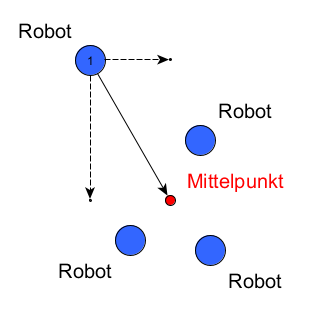
\includegraphics[width=\pictureWidth,keepaspectratio]{graphics/SchwarmMittelpunktBerechnung.png}
	\caption{Berechnung des Mittelpunkts}
	\label{pic:BerechnungMittelpunkt}
\end{wrapfigure}

Dieser Abschnitt wird realisiert indem ebenfalls zuerst die Roboter in eine Liste kopiert werden, die nahe genug sind um zur Nachbarschaft zu gehören. Anschließend wird ein simpler Durschnitt über alle Positionen (x/y - Koordinaten), der vorhandenen Roboter berechnet. Die resultierenden Koordinaten werden von den eigenen Koordinaten abgezogen, um die relative Position des Schwarm-Mittelpunkts zu bekommen. Indem man nun die relativen Koordinaten als Vektor behandelt und dadurch zu einem Winkel umrechnet, erhält man letztlich den relativen Winkel, den der Mittelpunkt der Nachbarschaft zum Roboter hat. Dieser Winkel wird mit normaler Geschwindigkeit angefahren.

Dabei ist der Mittelpunkt der Nachbarschaft wie er in~\autoref{pic:BerechnungMittelpunkt} zu sehen ist, allerdings nicht zwingend der Mittelpunkt der konvexen Hülle die die Nachbarschaft umgrenzt. Mehrere Roboter ziehen den Mittelpunkt der Nachbarschaft mehr in ihre Richtung. Der Vorteil dieser Methode ist schlicht, dass es den Roboter eher zu Gruppen zieht anderer Roboter zieht. Würde es den Roboter zur Mitte der konvexen Hülle ziehen, wäre die Gefahr groß, dass er alle Roboter verlieren würde, da sie zu allen Seiten gleich weit entfernt sind. Durch die einfache Methode des Mittelwerts bleibt der Roboter stets näher an Gruppen und lässt notfalls einzelne Roboter ziehen um die Gruppe zu behalten.

\subsubsection*{Abschottung: Vermeide Kollisionen mit deinen Nachbarn}

\begin{wrapfigure}{r}{\pictureWidth}
	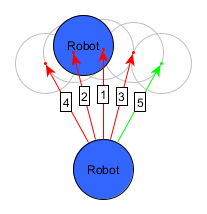
\includegraphics[width=\pictureWidth,keepaspectratio]{graphics/AusweichenAlgorithmus.png}
	\caption{Ausweichen gegenüber Hindernissen}
	\label{pic:AusweichenAlgorithmus}
\end{wrapfigure}

Damit die Roboter nicht beschädigt werden, müssen sie eine Größe erhalten und ihre Position mit der der anderen abprüfen. Eine Bewegung wird als gültig befunden, wenn der Roboter an seinem Zielpunkt mindestens seine Größe als Abstand zu allen anderen Robotern hat. Praktisch wurde die Größe um 10\per erweitert, um eine gewisse Fehlertoleranz zu erlauben.
Auch die Frequenz der in \autoref{subsec:NachbauNachrichten} erwähnten Positions-Nachrichten spielt hier wieder eine Rolle. 2 Roboter können dann aufeinander zufahren, wenn der Abstand beider Roboter nicht innerhalb der nächsten Aktualisierung der Positionsdaten überwunden werden kann.

Ob eine Kollision am Ziel (oder unterwegs) stattfinden wird, wird mittels interner Simulationen überprüft, die die letzten Positionsdaten der Roboter nutzt.
Findet eine Kollision statt, prüft der Roboter Ausweichmöglichkeiten. Der Algorithmus wird dabei angewendet, egal ob das Hinderniss ein anderer Roboter ist oder eine Gefahrenzone. Ist der Weg geradeaus nicht möglich, wird abwechselnd versucht nach links und rechts auszuweichen, wie in~\autoref{pic:AusweichenAlgorithmus} gezeigt wird. Dabei wird der Winkel, der zum Ausweichen genutzt, wird stufenweise erhöht, bis man letztlich 180° zu beiden Seiten erreicht hat, was einem Schritt rückwärts entspricht. Führt auch dieser letzte Winkel nicht zu einem erfolgreichen Ergebnis, wird der Algorithmus erneut mit einer leicht geringeren Geschwindigkeit (was ebenfalls einer leicht geringeren Bewegungsdistanz entspricht) gestartet. Erst wenn eine Simulation eine erfolgreiche Bewegung generieren konnte, wird diese auch ausgeführt.

\subsubsection*{Flucht: Fliehe vor Dingen, die eine potentielle Gefahr darstellen}

Gefahren wie Hindernisse, Löcher im Boden oder Zonen mit sich bewegenden Maschinen können die Roboter beschädigen, weshalb es gilt diesen Auszuweichen. Bei jeder Bewegung muss geprüft werden, ob man mit der angestrebten Bewegung eine Gefahrenzone betreten würde. Wenn ja, wird versucht mit dem Algorithmus des vorigen Abschnitts auszuweichen.

Um Gefahrenzonen abbilden zu können, werden Objekte erzeugt die sich aus verschiedenen Geometrien, mitsamt Positionen, zusammensetzen. Betritt ein Roboter eine der, im Objekt inneliegenden Geometrien, ist das Objekt als ganzes betreten worden und der Roboter befindet sich in einer Gefahrenzone.
Um ein Objekt zu definieren, ließen sich auch andere Methoden nutzen. Punkte die die Zone umspannen und eine konvexe Hülle bilden oder der Reihenfolge nach mit Geraden verbunden werden, wären ebenfalls eine Option. Allerdings wären diese viel komplexer zu berechnen und es würde unnötig Rechenleistung verbrauchen.
Die Berechnung, ob sich ein geometrischen Objekt innerhalb eines anderen geometrischen Objektes befindet, ist außerdem ein häufiges und gut gelöstes Problem von Videospielen.~\footnote{url{https://wwwx.cs.unc.edu/~geom/papers/documents/dissertations/lin93.pdf}}

\subsection*{Parameter der Bewegung}

Konfiguriert wird das Schwarmverhalten der Roboter durch 4 Parameter, die in den nachfolgenden Abschnitten näher erläutert werden.

\begin{wrapfigure}{r}{\pictureWidth}
	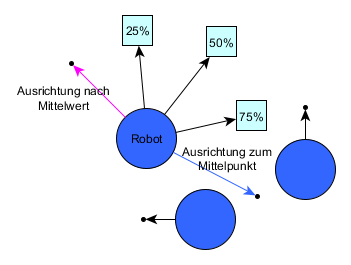
\includegraphics[width=\pictureWidth,keepaspectratio]{graphics/BerechnungDrangZurGruppe.png}
	\caption{Berechnung des Drangs zur Gruppierung}
	\label{pic:BerechnungDrangZurGruppe}
\end{wrapfigure}

\paragraph*{Geschwindigkeit} Gibt an, wie schnell ein Roboter sich bewegt. Ein kleinerer Wert sorgt für langsamere, aber auch 'vorsichtigere' Roboter. Optimal wäre ein kleiner Wert in Geschwindigkeit, aber eine hohe Frequenz an Bewegungs-Befehlen.

\paragraph*{Lokale Reichweite} Da ein Roboter nur seine unmittelbare Umgebung imitiert, braucht es dafür einen Grenzwert. In dieser Thesis wurde sich für eine Begrenzung in der Reichweite (im Gegensatz zu einer Begrenzung in der Anzahl der Roboter) entschieden, da die unmittelbare Umgebung wichtiger ist, als eine feste Anzahl an Robotern an denen sich orientiert wird. Einheiten die weiter weg sind als dieser Wert (in der entsprechenden Maßeinheit), werden für Berechnungen ignoriert. Ein Wert kleiner als die eigene physikalische Größe, führt zwangsläufig dazu, dass der Roboter nur sich selbst beachtet.

\paragraph*{Freier Wille} Einheiten im Schwarm orientieren sich nicht nur an seinen Nachbarn, sondern haben auch in gewisser Weise einen eigenen Willen. Nachdem die Berechnung der Orientierung am Schwarm abgeschlossen ist wird der eigene Wille einberechnet. Das ist ein Winkel der zufällig zwischen [-x/2, x/2] ausgesucht wird und dem bisherigen Winkel aufgerechnet wird.

\paragraph*{Nähe zum Schwarm} Dieser Wert ist verbunden mit der Regel 'Zusammenhang: Versuche deinen Nachbarn Nahe zu sein'. Ein Roboter hat den Drang seinem Schwarm nahe zu bleiben und versucht sich, bis zu einem gewissen Grad, in dessen Richtung zu bewegen. Da der Drang zum Schwarm nahe zu bleiben als Teil des freien Willens gezählt wird, wird dieser Wert prozentual angegeben und nach dem freien Willen auf den endgültigen Winkel aufgerechnet. Wie genau der Drang zur Gruppierung in Prozente eingeteilt ist, wird in \autoref{pic:BerechnungDrangZurGruppe} skizziert dargestellt.

\subsection*{Beispiel: Berechnung einer Bewegung}

\begin{wrapfigure}{r}{\pictureWidth}
	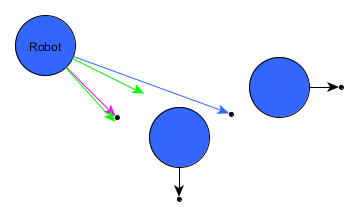
\includegraphics[width=\pictureWidth,keepaspectratio]{graphics/BerechnungBewegung.png}
	\caption{Berechnung einer Bewegung}
	\label{pic:BerechnungBewegung}
\end{wrapfigure}

In~\autoref{pic:BerechnungBewegung} ist die Berechnung einer Bewegung skizziert. Die Pfeile geben dabei nur Richtungen an und sind nicht als Vektoren zu verstehen, die eine Aussage über die bewegte Entfernung treffen.

Der pinke Pfeil ist das Resultat der Berechnung des Mittelwerts der Winkel, den die anderen Roboter beim letzten Update ihrer Position haben.

Der blaue Pfeil ist der Mittelpunkt des Schwarms (in diesem Fall sind beide Roboter ein Teil der Nachbarschaft), auf den der Roboter sich aufgrund seiner Gruppenzugehörigkeit zubewegen möchte.

Die beiden grünen Pfeile sind letztlich die obere und untere Grenze des Spielraums, den der Roboter durch seinen eigenen freien Willen bekommt. Dieser wurde durch die Ausrichtung zum Schwarm-Mittelpunkt zusätzlich leicht verschoben. Aus diesen beiden Grenzen wird letztlich ein Winkel zufällig bestimmt und anschließend auf Gültigkeit (fehlende Kollisionen) geprüft um dann schlussendlich ausgeführt zu werden.



\section{Anführer}

Um später Transportaufträge erledigen zu können, muss der Schwarm in irgendeiner Form gesteuert werden können. Bei einer direkten Steuerung aller Einheiten des Schwarms, wäre das Schwarmverhalten allerdings außer Kraft gesetzt und man hätte schlicht eine Menge gelenkter Roboter. Deswegen wurden Mittel gesucht den Schwarm indirekt zu lenken und fand diese Methode in einem Paper \note{QUELLE} in dem beschrieben wurde, wie ein Schwarm über 'eingeweihte Anführer' gesteuert werden kann.

Der Anführer bietet eine passive Möglichkeit einen Schwarm zu lenken, ohne dass die normalen Einheiten angepasst werden müssen oder in ihrem Verhalten speziell abweichen müssen. Die normalen Einheiten müssen dadurch nicht wissen, dass sie ein bestimmtes Ziel haben, es muss ihnen nicht einmal bewusst sein, dass sie passiv gesteuert werden. Dadurch, dass er stets in die Richtung des Ziels zeigt, aber auch aufgrund des Gruppendrangs durch die Nachbarn, pendeln sich die anderen Einheiten des Schwarms, langsam auf das Ziel ein. Ein Anführer ist somit eine Art Leuchtturm, der permanent eine Richtung angibt ohne sich von der Umwelt beeinflussen zu lassen und der den anderen Robotern eine Orientierung gibt.

Als Anführer versucht die entsprechende Einheit außerdem den Kontakt zu seiner Herde nicht zu verlieren. Damit ist nicht nur der Drang gemeint die Gruppenmitte aufzusuchen. Es ist eine bewusstere Art auf den eigenen Schwarm acht zu geben.

\subsection*{Ziel}

Ziel dieser Phase ist es, den Schwarm von einem Ort zu einem anderen zu lenken, ohne ihn wissen zu lassen dass er gelenkt wird. Dies soll mit Hilfe von (möglichst wenigen) Anführer geschehen die über das Ziel Bescheid wissen. Auf diese Weise muss nur wenig  in das ursprüngliche Verhalten der Roboter eingegriffen werden und der Schwarm bleibt möglichst natürlich.

\subsection*{Einbindung des Anführers in ROS}

Der Anführer wurde umgesetzt, indem einer normalen Einheit ein Ziel gegeben wird und er damit beginnt seinen Schwarm an einen bestimmten Ort zu lenken. Dazu werden die Roboter ein neues Topic abonnieren. Über dieses kann eine einfache Nachricht an einen bestimmten Roboter versendet werden. Dieser Roboter wird zum Anführer und hat versucht seinen Schwarm an die entsprechenden Koordinaten zu lenken.

\subsection*{Nachrichten}

Um den Transport einzuleiten wird es einen neuen Nachrichten-Typ geben. Die Nachricht kann an den Schwarm rausgesendet werden und durch die eindeutige ID weiß der entsprechende Roboter, dass er als Anführer ausgewählt wurde.

\begin{lstlisting}[style=ros, title=Nachrichten-Typ: New\_Mission]
	uint8	leader_id	// Die ID des ausgewaehlten Anfuehrers
	float32 pos_x		// Position des Ziels entlang der X-Achse
	float32 pos_y		// Position des Ziels entlang der Y-Achse
\end{lstlisting}

\subsection*{Generelles Verhalten}

Er steuert direkt auf das Ziel zu und wartet gegebenenfalls, wenn er sich zu weit vom eigenen Schwarm entfernt. Ab einer Entfernung von 75\per, der lokalen Reichweite zum Mittelpunkt seiner Herde, bleibt er stehen, bis er wieder bei 50\per Entfernung angekommen ist. Anschließend setzt er seinen Weg mormal fort. Ausweichmanöver würden dafür sorgen, dass der Anführer nicht mehr auf das Ziel zeigt und damit auch die anderen Roboter dazu bringen der neuen Ausrichtung zu folgen. Aus diesem Grund wird anderen Robotern nicht ausgewichen, wie es für Schwarmroboter üblich ist. Stattdessen wird der Anführer seine Geschwindigkeit verlangsamen, wenn er mit der normalen Geschwindigkeit eine Kollision verursachen würde. Kann er sich, trotz geringerer Geschwindigkeit nicht bewegen, bleibt er stehen und wartet eine kleine Zeitspanne ab.

\begin{wrapfigure}{r}{\pictureWidth}
	\includegraphics[width=\pictureWidth,keepaspectratio]{graphics/AlgorithmusAnführer.png}
	\caption{Entfernungen des Anführers}
	\label{pic:AnführerReichweiten}
\end{wrapfigure}

\subsubsection*{Einfangen eines verlorenen Schwarms}\label{subsubsec:AnführerEinfangen}
Sollte der Schwarm den Grenzbereich der lokalen Reichweite ganz verlassen, wäre es außerdem möglich, den Anführer seinen Schwarm wieder einfangen zu lassen. Dies ist in \autoref{pic:AnführerEinfangen} dargestellt.
Im ersten Abschnitt ist der Schwarm verloren gegangen, obwohl der Anführer gewartet hat. Anschließend ist er mit erhöhter Geschwindigkeit hinter den Schwarm gefahren, sodass der Schwarm sich nun genau zwischen Ziel und Anführer befindet. Nun nimmt er wieder sein normales Verhalten an und versucht den Schwarm in die Richtung des Ziel zu lenken. Beim umdrehen, um den Schwarm wieder einzufangen, dreht sich der Anführer allerdings in die entgegengesetzte Richtung. Die anderen Roboter wissen nichts von einem Manöver und orientieren sich normal am Anfüher. Das kann dazu führen, dass der Schwarm zunächst noch weiter abgelenkt wird. Aus diesem Grund sollte das Einfangen so schnell wie möglich beendet werden. Die Geschwindigkeit des Anführers sollte also möglichst hoch sein.

\begin{wrapfigure}{r}{\pictureWidth}
	\includegraphics[width=\pictureWidth,keepaspectratio]{graphics/AlgorithmusAnführerEinfangen.png}
	\caption{Anführer fängt seinen Schwarm wieder ein}
	\label{pic:AnführerEinfangen}
\end{wrapfigure}


% ====================================================================================================
% ====================================================================================================
% ====================================================================================================






\section{Transport von Waren mit Hilfe eines Schwarms}

Das letztliche Ziel dieser Arbeit ist es zu prüfen, ob es möglich, und sinnvoll, ist Gegenstände mit Hilfe eines autonomen Schwarms zu transportieren. Dazu musste der Schwarm nun dazu gebracht werden Waren zu bewegen, ohne die einzelnen Roboter zu sehr zu beeinflussen. Da generell die Roboter nicht zentral gesteuert werden sollen und auch die Logik möglichst simple bleiben soll, sollte das Programm der einzelnen Einheiten möglichst wenig verändert werden und der 'natürliche' Trieb der Einheiten genutzt werden.

\subsection*{Erteilen von Aufträgen}

Eine der ersten Dinge im Ablauf eines Transports ist die Erteilung des Auftrags. Dazu muss der Nachrichten-Typ \highlight{New\_Mission} im ROS-Netzwerk erweitert werden, sodass er nun die folgenden Felder hat:

\begin{lstlisting}[style=ros]
uint8 robot_index_from		// Beginn der ID-Range
uint8 robot_index_to		// Ende der ID-Range

uint8 leader_number			// Anzahl der Leader die gebraucht werden
uint8 mission_id			// Die ID der Mission

float32 object_position_x	// Die Start-Position des Transport-Objektes, X-Achse
float32 object_position_y	// Die Start-Position des Transport-Objektes, Y-Achse

float32 object_size_x		// Die Laenge des Objektes, in X-Richtung
float32 object_size_y		// Die Laenge des Objektes, in Y-Richtung

float32 target_x			// Die Ziel-Position des Transport-Objektes, X-Achse
float32 target_y			// Die Ziel-Position des Transport-Objektes, Y-Achse
\end{lstlisting}

Der Nachrichten-Typ definiert nun eine Spanne von Robotern die den Auftrag ausführen sollen. Diese werden mit ihren IDs angesprochen. Das Intervall der IDs ist, gemäß Programmierstandards, als halboffenes Intervall definiert: [robot\_index\_from, robot\_index\_to[.
leader\_number gibt die Anzahl der Leader an die verwendet werden sollen und mission\_id gibt dem derzeitigen Auftrag eine fixe ID um diesen und zugehörige Dinge genau identifizieren und verbinden zu können.
Mit object\_position\_x/-\_y ist die Startposition des zu transportierenden Objektes angegeben. Zusammen mit object\_size\_x/-\_y, welche die Ausmaße des Objektes angeben. Die Position des Objekts ist als Mitte des Objekts definiert.
target\_x/-\_y gibt die letztliche Position an die das Objekt einnehmen soll.

Der Auftrag wird von außen an das Topic 'flock/mission/new' gesendet. Der Ersteller des Auftrags muss keine ROS-Node sein, auch wenn dies verschiedene Vorteile hätte. Dadurch das ROS-Topics auch über das Terminal engesprochen werden können, ist das Senden der Nachrichten auch über jedes andere Programm möglich. Das Topic für die neuen Missionen wird von jedem aktiven Roboter abonniert. Entsprechend nimmt jeder Roboter Notiz von diesem Auftrag, auch wenn er nicht direkt mit seiner ID angesprochen wird.

\subsection*{Von Gefahrenzonen zu Sicherheitszonen}

Um die betreffenden Roboter in die Zone zu senden, auf der ihnen später das Transportobjekt aufgesetzt wird, wird ein Mechanismus verwendet der bereits vorher Einzug in das ROS-System hielt: Gefahrenzonen. Diese werden leicht angepasst, um sie invertieren zu können und somit aus einer Gefahrenzone eine Sicherheitszone zu machen. Ist ein Bereich als Sicherheitszone definiert, ist jeder andere Bereich automatisch eine Gefahrenzone.
Dieser Mechanismus birgt nur eine kleine Änderung im System, schafft es aber Roboter in einen bestimmten Bereich zu locken ohne sie aktiv steuern zu müssen, indem einfach ihr 'natürlicher' Trieb verwendet wird, von Gefahren zu flüchten.

Wird ein Auftrag erteilt, so nehmen die Roboter die dem Auftrag zugeteilt sind, eine neue Sicherheitszone auf, die den Ausmaßen und der Position des Transportobjekts am Aufnahmeort entsprechen. Roboter die nicht dem Transport zugeteilt wurden, werden diese neue Zone als Gefahrenzone auffassen und versuchen sich diesem Gebiet fernzuhalten.

Ein Objekt kann grundsätzlich aus verschiedenen Geometrien zusammengesetzt werden. Dadurch ist es möglich nicht nur Objekte zu transportieren die eine einfache Form wie Rechtecke oder Kreise haben, sondern verschiedene Rechtecke können dann zu einem 'L' oder 'U' zusammengesetzt werden.

\subsection*{Füllen eines Raums}

Wird eine Sicherheitszone definiert, versuchen die Roboter, die sich in der Gefahrenzone befinden, auf möglichst schnellstem Wege die Sicherheitszone zu betreten. Dazu wird das Zentrum der Sicherheitszone ins Ziel genommen und (ohne mit anderen Robotern zu kollidieren) der direkte Weg darauf zu genommen. Dabei kann es dann allerdings vorkommen, dass eine komplexere Form nicht vernünftig gefüllt werden kann, oder dies sehr lange dauert. Da ein eintreffender Roboter so lange auf den Mittelpunkt zufahren würde, bis die Roboter darin sich genug verteilt haben um genug Platz für den neuen Roboter zu schaffen.

Ein Algorithmus, wie man es schafft mit Roboter einen definierten Raum zu füllen, lässt sich in (\note{HIER; QUELLE}) finden. Dieser Algorithmus lässt sich aufgrund anderer Fähigkeiten bei den Robotern und dem gewünschten Schwarmverhalten nicht vollständig nachbilden. Eine andere, bereits implementierte Fähigkeit, lässt sich dagegen gut nutzen um den Algorithmus annähernd nachzubauen: Ausweichen.

\begin{wrapfigure}{r}{\pictureWidth}
	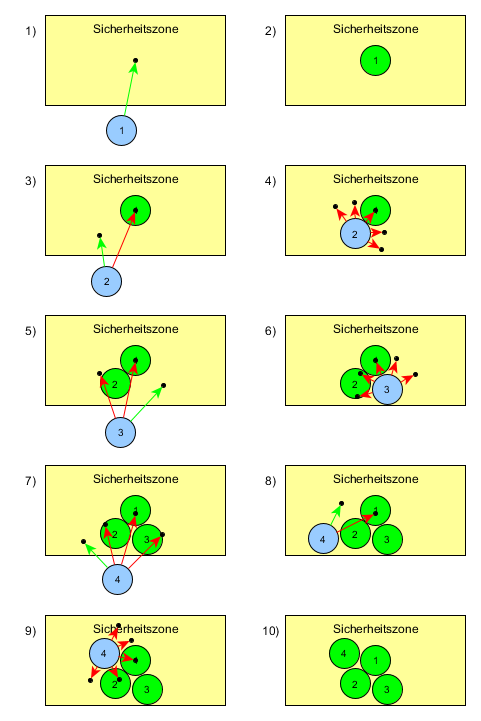
\includegraphics[width=\pictureWidth,keepaspectratio]{graphics/AlgorithmusAusweichenTransport.png}
	\caption{Roboter füllen das Transportobjekt}
	\label{pic:AlgorithmusAusweichenObjekt}
\end{wrapfigure}

Betritt ein Roboter die Sicherheitszone des Transport-Objekts, reduziert dieser seine Geschwindigkeit und fährt langsam weiter auf den Mittelpunkt zu. Neu ankommende Roboter werden durch die vorderen, viel langsameren Roboter zum Ausweichen gezwungen, was letztlich dazu führt, dass die Roboter sich seitlich verteilen, aber langfristig den Nachfolgern Platz machen. Ist ein Roboter nahe genug am Mittelpunkt angekommen oder findet in einem Umkreis von [-90°, 90°] keinen Platz mehr der näher am Mittelpunkt ist als der aktuelle, bleibt er stehen. Roboter die stehen bleiben senden den anderen Robotern ihres Schwarms ein entsprechendes Signal dass sie bereit sind. Haben alle Roboter erkannt dass die anderen bereit sind, ist die Phase des Eintreffens am Abnahmepunkt abgeschlossen.

Von hier an braucht es ein Event, dass den Robotern zeigt dass sie mit dem Transportobjekt Richtung Ziel losfahren können. Möglich wäre eine Zeitsteuerung für streng automatisierte Prozesse. Aber auch interne Signale über ROS sind möglich. Durch die ID die jeder Auftrag hat, wäre eine einfache Nachricht '[TransportID\#][Losfahren]' bereits zielführend.

\paragraph*{Der Algorithmus am Beispiel}
\autoref{pic:AlgorithmusAusweichenObjekt} zeigt den Algorithmus anhand eines Beispiels mit 4 Robotern.

Der erste Roboter versucht zur Mitte des Objekts zu gelangen und findet sofort Zugang zum Objekt. Er reduziert seine Geschwindkeit und platziert sich langsam im Mittelpunkt des Objektes. Da seine Nähe zum Mittelpunkt klein genug ist, bleibt er letztlich stehen.

Der nächste Roboter kommt, wird allerdings von seinem Vorgänger leicht blockiert. Das führt dazu dass dieser versucht nach links auszuweichen und damit Erfolg hat. Er betritt die Zone, findet aber keinen besseren Ort und bleibt daraufhin stehen.

Der dritte Roboter wird ebenfalls von seinen Vorgängern blockiert, findet aber rechts eine Stelle. Nachdem er diese eingenommen hat findet auch er keine bessere Stelle und bleibt ebenfalls stehen.

Der vierte Roboter findet zunächst links eine Stelle und betritt daraufhin die Zone. Er verlangsamt seine Bewegung und sucht nun nach Stellen die ihn ohne Kollisionen näher zu seinem Ziel führen, wobei er einmal Roboter\#2 umkreist. In der Lücke zwischen Roboter\#2 und Roboter\#1 findet er die beste Stelle und bleibt dort anschließend stehen. Der Algorithmus für diese 4 Roboter ist damit abgeschlossen. Sie stehen alle in der Fläche des Transportobjektes und stehen still, bereit die Lieferung entgegen zu nehmen.

\subsection*{Der Transport}

Um den Transport selbst zu realisieren bedient man sich der Hilfe der Anführer. Diese richten sich dynamisch nach dem Winkel aus, den das Transportobjekt zum Ziel hat, wie \autoref{pic:AlgorithmusTransport} zeigt. Danach fangen sie an sich langsam in die Richtung zu bewegen in die sie sich ausgerichtet haben. Die anderen Roboter werden sich aufgrund des Gruppenverhaltens ebenfalls mehr oder weniger nach ihren Anführern ausrichten und das Objekt so langsam Richtung Ziel bewegen.

\begin{wrapfigure}{r}{\pictureWidth}
	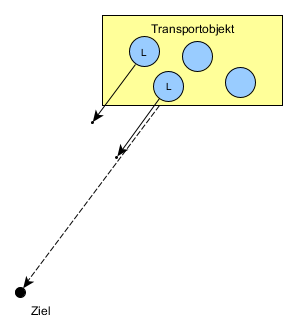
\includegraphics[width=\pictureWidth,keepaspectratio]{graphics/AlgorithmusTransport.png}
	\caption{Der Transport des Objekts}
	\label{pic:AlgorithmusTransport}
\end{wrapfigure}

\subsubsection*{Einhalten der Richtung hat Priorität}

Kann ein Anführer keine normale Bewegung ausführen, weil er sonst mit einem anderen Roboter kollidieren würde, darf er nicht versuchen auszuweichen, da dies sonst die Ausrichtung der passiven Roboter negativ beeinflussen könnte. Stattdessen drosselt er zunächst sein Bewegungstempo oder bleibt, falls notwendig, ganz stehen. Die richtige Richtung beizuhalten ist wichtig, da sich passive Roboter nicht unmittelbar nach ihren Anführern ausrichten. Gerade wenn es zahlenmäßig wenige Anführer im Vergleich zu passiven Robotern sind, kann es einige Zeit dauern, bis die Einheiten so weit beeinflusst wurden, dass sie in die gewünschte Richtung zeigen. Dreht sich ein Anführer in die verkehrte Richtung, vielleicht sogar in die entgegengesetzte, kann dies zu einer Kettenreaktion führen die alle Roboter betrifft und zusätzlich das Transportobjekt stark vom Weg abbringen. Dieser Effekt konnte bereits in früheren Simulationen erkannt werden (siehe: \autoref{subsec:AnalyseNachbesserung}}) und wird deshalb in dieser Konzeption vermieden.

\subsubsection*{Abschluss des Transports}






